\documentclass[12pt,oneside,a4paper,parskip]{scrbook}
\usepackage[utf8]{inputenc}
\usepackage{csquotes}
\usepackage[ngerman]{babel}
\usepackage{floatflt}
\usepackage{subfigure}
\usepackage[pdftex]{graphicx}
\usepackage[hidelinks]{hyperref}
\usepackage{color}
\usepackage{amssymb}
\usepackage{textcomp}
\usepackage{nicefrac}
\usepackage{scrhack}
\usepackage{pdfpages}
\usepackage{float}
\usepackage{pdflscape}
\usepackage{subfigure}
\usepackage{pdfpages}
\usepackage[verbose]{placeins}
%\usepackage[nouppercase,headsepline,plainfootsepline]{scrpage2}
\usepackage{listings}
\usepackage{xcolor}
\usepackage{color}
\usepackage{caption}
\usepackage{subfigure}
\usepackage{epstopdf}
\usepackage{longtable}
\usepackage{setspace}
\usepackage{booktabs}
\usepackage[style=numeric,backend=biber, uniquelist=false]{biblatex}
\bibliography{literatur}
\addbibresource{literatur.bib}


%%%%%%%%%%%%%%%%%%%
%% definitions
%%%%%%%%%%%%%%%%%%%
\def\BaAuthor{David Mödl\, Sebastian Lober}
\def\BaAuthorStudyProgram{Informatik} %% Wirtschaftsinformatik, E-Commerce, Informationssysteme
\def\BaType{Seminararbeit} %% Masterarbeit
\def\BaTitle{Bias of Neural Networks - Security implications}
\def\BaSupervisorOne{Prof.\ Dr.\ A B}
\def\BaSupervisorTwo{Prof.\ Dr.\ C D}
\def\BaDeadline{\today}

\ifdefined\iswithfullname
  \def\ShowBaAuthor{\BaAuthor}
\else
  \def\ShowBaAuthor{N.~N.}
\fi

\hypersetup{
pdfauthor={\ShowBaAuthor},
pdftitle={\BaTitle},
pdfsubject={Subject},
pdfkeywords={Keywords}
}

%%%%%%%%%%%%%%%%%%%
%% configs to include
%%%%%%%%%%%%%%%%%%%
\colorlet{punct}{red!60!black}
\definecolor{background}{HTML}{EEEEEE}
\definecolor{delim}{RGB}{20,105,176}
\colorlet{numb}{magenta!60!black}

\definecolor{gray}{rgb}{0.4,0.4,0.4}
\definecolor{darkblue}{rgb}{0.0,0.0,0.6}
\definecolor{cyan}{rgb}{0.0,0.6,0.6}

\definecolor{pblue}{rgb}{0.13,0.13,1}
\definecolor{pgreen}{rgb}{0,0.5,0}
\definecolor{pred}{rgb}{0.9,0,0}
\definecolor{pgrey}{rgb}{0.46,0.45,0.48}

\lstset{
  basicstyle=\ttfamily,
  columns=fullflexible,
  showstringspaces=false,
  commentstyle=\color{gray}\upshape
  linewidth=\textwidth
}

\lstdefinelanguage{json}{
    basicstyle=\normalfont\ttfamily,
    numbers=left,
    numberstyle=\scriptsize,
    stepnumber=1,
    numbersep=8pt,
    showstringspaces=false,
    breaklines=true,
    backgroundcolor=\color{background},
    literate=
     *{0}{{{\color{numb}0}}}{1}
      {1}{{{\color{numb}1}}}{1}
      {2}{{{\color{numb}2}}}{1}
      {3}{{{\color{numb}3}}}{1}
      {4}{{{\color{numb}4}}}{1}
      {5}{{{\color{numb}5}}}{1}
      {6}{{{\color{numb}6}}}{1}
      {7}{{{\color{numb}7}}}{1}
      {8}{{{\color{numb}8}}}{1}
      {9}{{{\color{numb}9}}}{1}
      {:}{{{\color{punct}{:}}}}{1}
      {,}{{{\color{punct}{,}}}}{1}
      {\{}{{{\color{delim}{\{}}}}{1}
      {\}}{{{\color{delim}{\}}}}}{1}
      {[}{{{\color{delim}{[}}}}{1}
      {]}{{{\color{delim}{]}}}}{1},
}

\lstset{language=xml,
  morestring=[b]",
  morestring=[s]{>}{<},
  morecomment=[s]{<?}{?>},
  stringstyle=\color{black},
  numbers=left,
  numberstyle=\scriptsize,
  stepnumber=1,
  numbersep=8pt,
  identifierstyle=\color{darkblue},
  keywordstyle=\color{cyan},
  backgroundcolor=\color{background},
  morekeywords={xmlns,version,type}% list your attributes here
}

\lstset{language=Java,
  showspaces=false,
  showtabs=false,
  tabsize=4,
  breaklines=true,
  keepspaces=true,
  numbers=left,
  numberstyle=\scriptsize,
  stepnumber=1,
  numbersep=8pt,
  showstringspaces=false,
  breakatwhitespace=true,
  commentstyle=\color{pgreen},
  keywordstyle=\color{pblue},
  stringstyle=\color{pred},
  basicstyle=\ttfamily,
  backgroundcolor=\color{background},
%  moredelim=[il][\textcolor{pgrey}]{$$},
%  moredelim=[is][\textcolor{pgrey}]{\%\%}{\%\%}
}

\newcommand*{\forcetwosidetitle}[1][1]{%
 \begingroup
   \cleardoubleoddpage
   \KOMAoptions{titlepage=true}% useful e.g. for scrartcl
   \csname @twosidetrue\endcsname
   \maketitle[{#1}]
 \endgroup
}


\begin{document}


%%%%%%%%%%%%%%%%%%%
%% Titelseite
%%%%%%%%%%%%%%%%%%%


\frontmatter
\titlehead{%  {\centering Seitenkopf}
  {Hochschule für angewandte Wissenschaften Würzburg-Schweinfurt\\
   Fakultät Informatik und Wirtschaftsinformatik}}
\subject{\BaType}
\title{\BaTitle\\[15mm]}
%\subtitle{\normalsize{vorgelegt an der Hochschule f\"{u}r angewandte Wissenschaften W\"{u}rzburg-Schweinfurt in der Fakult\"{a}t Informatik und Wirtschaftsinformatik zum Abschluss eines Studiums im Studiengang \BaAuthorStudyProgram}}
\author{David Mödl \& Sebastian Lober}
%\date{\normalsize{Eingereicht am: \BaDeadline}}
%\publishers{
%  \normalsize{Erstpr\"{u}fer: \BaSupervisorOne}\\
%  \normalsize{Zweitpr\"{u}fer: \BaSupervisorTwo}\\
%}
\forcetwosidetitle


%%%%%%%%%%%%%%%%%%%
%% abstract
%%%%%%%%%%%%%%%%%%%

\section*{Zusammenfassung}
Künstliche Intelligenz (KI) ist eines der Gesprächsthemen beim Umstieg in die Industrie 4.0. Trotz des ganzen Hypes um das Thema, gibt es zahlreiche Herausforderungen die dabei gemeistert werden müssen.
\\\\
Eine dieser Herausforderung nennt sich KI-Bias. Das Ziel dieser Arbeit ist es ein allgemeines Verständnis, wie KI-Bias auftreten und vermieden werden können, zu vermitteln. Anhand konkreter Beispiele wird die Entstehung solcher Bias gezeigt. Im Abschluss werden Präventionen dagegen aufgezeigt.\\
Außerdem soll dem Lesern ein Grundwissen über Sicherheitsrisiken für Mensch und Maschine, solcher KI-System vermittelt werden.
\\\\
Die Arbeit bezieht sich auf mehrere wissenschaftliche Arbeiten und ist meist mit solchen belegt worden.

%%%%%%%%%%%%%%%%%%%
%% Inhaltsverzeichnis
%%%%%%%%%%%%%%%%%%%
\tableofcontents



%%%%%%%%%%%%%%%%%%%
%% Main part of the thesis
%%%%%%%%%%%%%%%%%%%
\mainmatter

\chapter{Einführung}
\label{chapter:intro}
Künstliche Intelligenz(KI) oder auch artifizielle Intelligenz(AI) tritt allgegenwärtig in großen Teilen unserer Gesellschaft auf. Von Kaufvorschlägen auf Amazon, über Chat-Bots bis hin zu autonom fahrenden Autos spielt die KI eine immer größere Rolle. Ein bekanntes Beispiel ist die Software AlphaGo, die als erstes Computer Programm 2016 den weltbesten Profispieler im komplexen Brettspiel Go besiegen konnte\cite{alphaGo}. Darüber hinaus ermöglicht die KI komplexe Sachverhalte zu simulieren und zu prognostizieren, wie zum Beispiel die vollautomatische Generierung hochaufgelöster, realistischer Videosequenzen auf der Grundlage simpler Eingaben\cite{videoToVideo}.
\\\\
Einerseits gibt es viele Erfolge, die für ein KI betriebenes System sprechen. Andererseits bestärken medienwirksame Verfehlungen, wie z.B. das frauenfeindliche Bewerbungssystem von Amazon\cite{amazon}, die Skeptiker solcher Systeme. Ziel dieser Arbeit ist es, die unterschiedlichen Ursprünge solcher algorithmischen Verzerrungen (engl. bias) zu erläutern und Präventionen zu schildern, welche diese vermeiden sollen.
\\\\
Wir beginnen unsere Arbeit damit, Grundlagen für ein fundamentales Wissen spätere Kapitel aufzubauen. Danach möchten wir auf die Entstehung solcher Bias eingehen, die damit verbundenen Probleme und welche Präventionen gegen diese Fehlverhalten unternommen werden können.
\chapter{Grundlagen}
\section{Bias}
Wesentlicher Bestandteil der Arbeit ist das Erläutern der "Biases", welche durch die Nutzung von künstlicher Intelligenz auftreten können. Das Wort Bias kommt aus dem Englischen und bedeutet im Wesentlichen:
\begin{enumerate}
	\item Verzerrung – im statistischen Sinn als mittlere systematische Abweichung zwischen dem erwarteten und dem tatsächlichen Modellergebnis. % Nochmal drüber nachdenken
	\item Voreingenommenheit – je nachdem, wie wir die Welt aufgrund unserer Erfahrungen sehen, kommen wir zu unterschiedlichen Schlüssen. % Nochmal drüber nachdenken
\end{enumerate}

Der Begriff Voreingenommenheit muss bei der Nutzung von KI vorsichtig behandelt werden, denn eine Maschine besitzt grundsätzlich keinerlei Vorurteile und weiß zu Beginn nicht was richtig oder falsch ist. Hier spricht man daher von einem Fehlverhalten oder einer Verzerrung, wie diese Entstehen werden im Kapitel \ref{chapter:BiasEntstehung} erläutert.
\section{Künstliche Intelligenz}
Künstliche Intelligenz(KI) oder auch artifizielle Intelligenz(AI) ist der Oberbegriff für ein Teilgebiet der Informatik. Dieses Gebiet befasst sich mit jeglicher Form von maschinelle intelligenten Verhalten und dem maschinellen Lernen, siehe Abbildung \ref{fig:Uebersicht}. Generell wird bei der künstlichen Intelligenz versucht biologische Intelligenz auf einen Computer zu simulieren. Dies basiert meist auf simplen Algorithmen, wodurch die Begrifflichkeit 'Intelligenz' in Bezug auf Maschinen öfter in Frage gestellt wird. \cite{Grundlagen}
\begin{figure}[ht]
	\begin{center}
		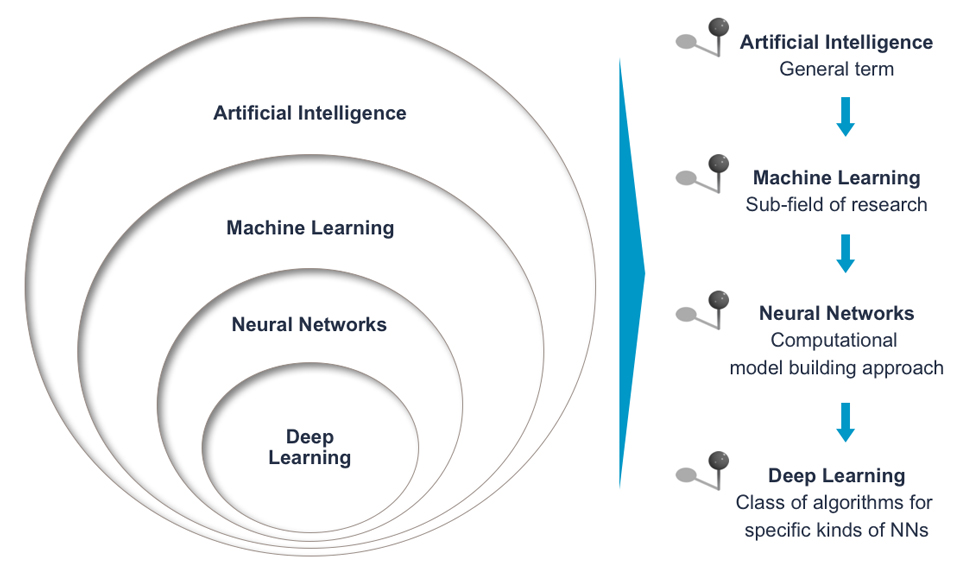
\includegraphics[width=14cm]{Bilder/Abstraktionslevel_von_AI.jpg}
		\caption{Verschiedene Abstraktionslevel von Artificial Intelligence in hierarchischer Ordnung}
		\label{fig:Uebersicht}
	\end{center}
\end{figure}
%https://www.capgemini.com/de-de/2017/09/artifical-intelligence-machine-learning-und-data-science-same-same-but-different/
\\\\Damit ein Programm den Titel KI tragen darf, muss sie zum einen die Fähigkeit zu lernen besitzen, zum anderen die Fähigkeit auch bei nicht eindeutigen Eingaben intelligent Lösungen zu finden.\\
KIs werden grob in zwei Kategorien aufgeteilt.\\
Die starke KI besitzt eine Intelligenz, die dem eines Menschens eben würdig ist bzw. sogar übersteigt. Ob eine starke KI überhaupt jemals erreicht wird, ist sehr umstritten. \\Schwache KI hingegen sind in unserem Alltag bereits vertreten. Schwache KI sind Algorithmen, die ganz spezielle Aufgaben lösen und die Arbeit von Menschen unterstützen.

\subsection{Maschine Learning}
Machine Learning (ML) ist der Oberbegriff jeglicher Lernformen von künstlicher Intelligenz. Im Allgemeinen versucht eine KI neue Muster und Gesetzmäßigkeiten in Trainingsdaten zu erkennen, diese zu verallgemeinern und für neue Problemlösungen oder für die Analyse von bisher unbekannten Daten zu verwenden\cite{EliminateHumanBias}.
\\\\Diese Arbeit speziell konzentriert sich auf Deep Learning, welches eine Variante zum Trainieren von neuronalen Netzen darstellt.
\subsubsection{Lernformen}
KIs bestehen aus vielen Algorithmen. Damit eine KI lernt, müssen diese Algorithmen angepasst werden. Hierbei gibt es drei übergeordnete Lernformen: überwachtes, unüberwachtes oder bestärkendes Lernen. \\\\
Beim überwachten Lernen sind Trainingsdaten bereits kategorisiert. Nach dem Versuch die Daten eigenständig zu kategorisieren, erhält das KI-System ein positives oder negatives Feedback. Auf Basis des Feedbacks lernt die KI, auf welche Muster und Merkmale es achten muss, um die Aufgabe richtig zu lösen\cite{Grundlagen}. \\
Die andere Variante ist das unüberwachte Lernen. Hierbei sind die Trainingsdaten nicht kategorisiert und das KI-System kann somit kein Feedback bekommen. Das neuronale Netz erstellt ein statisches Model aus den Trainingsdaten und versucht Zusammenhänge und wiederkehrende Muster zwischen den Daten zu erkennen. Zusammenhängende Daten werden einer Kategorie zugeordnet. Die lernende KI weiß zu keiner Zeit, ob das was es Gruppiert auch zusammengehört\cite{Grundlagen}.\\
Bestärkendes Lernen (auch Reinforcement Learning) ist eine Lernmethode bei dem der Algorithmus durch Belohnung und Bestrafung trainiert wird. Hierbei erhält das KI-System Feedback in Form von Belohnung bei Erfolg und Bestrafung, falls das bestimmte Verhalten nicht zielführend war. Mit dieser Lernmethode wurde Google AlphaGo trainiert\cite{Grundlagen}.
%%% Bestärkendes Lernen überdenken
\subsection{Neuronale Netze}
Künstliche neuronale Netze(KNN) bestehen aus künstlichen Neuronen, die untereinander verflechtet sind. Diese Konstrukte sind denen der sich im Nervensystem eines Lebewesens befindenden Neuronenverbindungen nachempfunden. \\
KNNs sind nicht dazu da das Nervensystem von Lebewesen nachzubilden, sondern abstrakt die Eigenschaften der Informationsverarbeitung und der Lernfähigkeit zu imitieren.
\begin{figure}[h]
	\begin{center}
		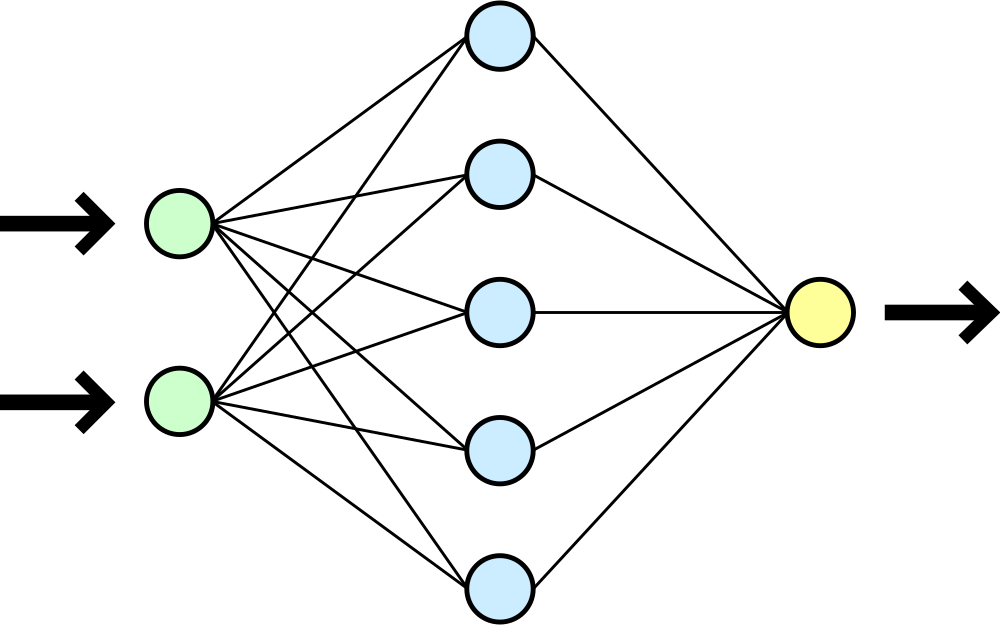
\includegraphics[width=10cm]{Bilder/Neurales_Netz.png}
		\caption{Vereinfachte Darstellung eines künstlichen neuronalen Netzes}
		\label{fig:wikiNeuronalesNetz}
	\end{center}
\end{figure}
% https://de.wikipedia.org/wiki/K%C3%BCnstliches_Neuron#/media/Datei:ArtificialNeuronModel_deutsch.png
\\\\KNNs sind meist in Schichten mit beliebig vielen künstlichen Neuronen aufgebaut. In der Regel besteht ein KNN aus drei Teilen die Eingangsschicht (grün), verdeckte Schicht (blau) im Englischen Hidden Layer und die Ausgabeschicht (gelb). In der Eingangsschicht fließen die Informationen in das Netz ein und in der Ausgabeschicht das Ergebnis der Berechnungen aus. Jede Schicht besteht aus beliebig vielen Neuronen je nach Komplexität des Zieles, die Hidden Layer sogar aus beliebig viele Schichten.
\\\\
In der Regel arbeiten KNNs nach dem feedforward-Prinzip, bei dem die Informationen nur in eine Richtung fließen. Es gibt jedoch auch rekurrente Netze, bei denen durch rückgerichtete Kanten Rückkopplungen im Netz entstehen. \\
Die einfachste Netzstruktur ist das einschichtige feedforward-Netz. Dies besteht ohne Rückkopplungen aus nur einer Schicht, der Ausgabeschicht.
\subsubsection{Das künstliche Neuron}
Künstliche Neuronen sind die Grundbestandteile eines künstlichen neuronalen Netzes.
Ein künstliches Neuron ist die vereinfachte und abstrakte Version einer biologischen Nervenzelle und ist wie folgt aufgebaut.\\\\
\begin{figure}[h]
	\begin{center}
		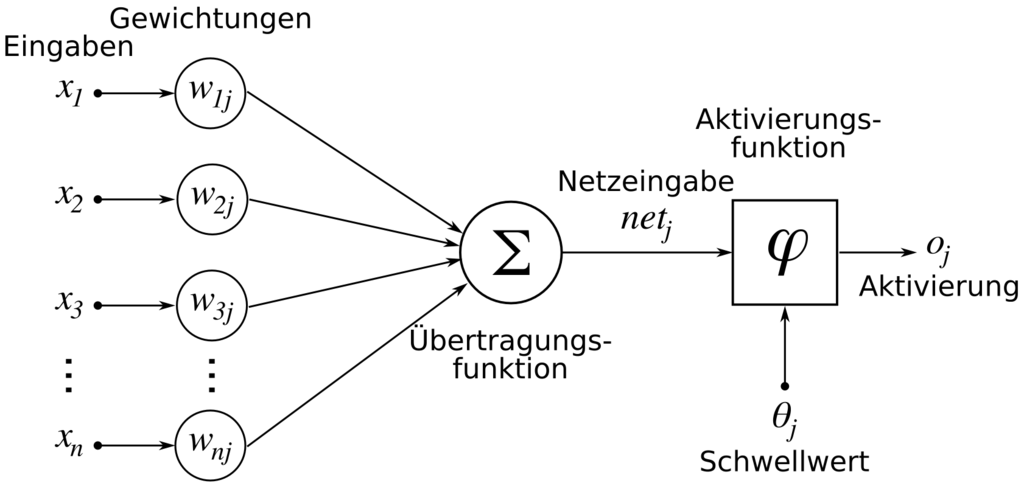
\includegraphics[width=12cm]{Bilder/ArtificialNeuronModel_deutsch.png}
		\caption{Ein künstliches Neuron}
		\label{fig:wikiNeuron}
	\end{center}
\end{figure}
% https://de.wikipedia.org/wiki/K%C3%BCnstliches_Neuron#/media/Datei:ArtificialNeuronModel_deutsch.png
Ein künstliches Neuron besitzt $n$ Eingangskanäle und einen Ausgangskanal. $j$ repräsentiert hier die eindeutige Nummer des Neuron. Jede Eingabe $x_{i}$ besitzt ein dazugehörendes Gewicht $w_{1j}..w_{nj}$. Dieser spiegelt die Wichtigkeit der Eingabe wider, welche hemmend (negativer Wert) oder erregend (positiver Wert) wirken kann. Die Übertragungsfunktion $\Sigma$ summiert alle multiplizierten Eingaben mit ihrem Gewicht und geht als Netzeingabe $net_j$ in die Aktivierungsfunktion $\varphi$ ein. \\
Ob das Neuron "'feuert"' oder kein Signal sendet, wird hier berechnet. Auf die Netzeingabe $net_j$ wird ein Schwellenwert $\theta_j$ addiert. Als mathematisch Vereinfachung wird der Schwellwert $\theta$ als $w_0$ bezeichnet und $x_0 = 1$ eingeführt und somit in der folgenden Formel immer auf die Netzeingabe $net_j$ addiert.
\\\\
${\displaystyle a=\sum _{i=0}^{n}x_{i}w_{i}}$
\\\\
Die Variabel $a$ geht in die Aktivierungsfunktion ${\sigma (a)}$ ein, anhängig von dem Ergebnis wird das Neuron aktiv oder bleibt inaktiv.
Das Ausgangssignal eines Neuron ist gleichzeitig ein Eingangssignal eines oder mehreren anderen Neuronen. %%% Den Satz nochmal überprüfen
\\\\
Dadurch dass ein Neuron mehrere Eingangskanäle besitzt, werden viele Eingangsinformationen auf ein Ergebnis reduziert. Durch mehrere Schichten und vielen Neuronen pro Schicht kann so eine große Menge an Daten schnell reduziert werden.
\\\\
Jedoch muss jedes künstliche Neuron eines KNNs richtig eingestellt werden, damit das KNN dessen Ziel erfüllt. Eingestellt wird das Neuron durch Training. Trainieren bedeutet hier das Ermitteln der richtigen Werte für Gewichtungen und Schwellwerte, als auch das Einstellen der richtige Verbindungskombinationen der Neuronen untereinander. Diesen Prozess nennt man Deep Learning, eine Form von Machine Learning.
\subsection{Deep Learning}
Deep Learning ist eine Maschine Learning Variante, die speziell bei künstliche neuronale Netze eingesetzt wird. Beim Deep Learning werden die zahlreichen Zwischenschichten der Hidden Layer trainiert. Dabei wird eine umfangreiche und komplexe Struktur der Neuronen-Verbindungen aufgebaut. Wie das Programm endgültig die Aufgabe lösen soll, wird hierbei nicht vorgegeben, sondern bei diesem autonomen Prozess evolutionär ermittelt\cite{Grundlagen}.
\\\\
Ein künstliches neuronales Netz wird mit dem Zweck aufgebaut, eine bestimmte Aufgabe zu lösen. Extra dafür müssen Daten aufbereitet werden. Aus diesen Daten werden Muster und Gesetzmäßigkeiten extrahiert, um Erfahrungen zu sammeln. Aus Basis dieser Erfahrungen werden später Entscheidungen auf unbekannte Daten angewandt \cite{Grundlagen}.
\\\\
Damit es ausgeschlossen ist, dass das Netz zufällige Zusammenhänge zwischen den Daten findet, wird eine hinreichend große Datenmenge, abhängig von der Komplexität, benötigt. Auch die Qualität der Daten ist entscheidend, da daraus der KI-System die fachlich Korrekten Schlüsse zieht, siehe Abschnitt \ref{section:Data}.
\\\\
Neuronale Netze sind für Menschen ab einer gewissen Größe nicht mehr nachvollziehbar. Somit kann nur die Eingabe mit der Ausgabe verglichen werden, um die Korrektheit der Aufgabenlösung zu prüfen. Ziel ist es mit möglichst vollständigen Trainingsdaten das Netzwerk so einzustellen, dass diese unbekannt Daten korrekt interpretiert \cite{Grundlagen}.
\\\\
Um eine Aufgabe zu trainieren, wird nicht nur ein Netz mit Zufallswerten und Verbindungen generiert sondern tausende. Beim überwachten Lernen werden alle mit den gleichen Trainingsdaten trainiert und mit den Testdaten geprüft. Für jedes Netz wird ein Mittelwert über die Korrektheit der Antworten erstellt. Da alle Netze Initial mit Zufallswerten belegt sind, haben die meisten Netze eine Erfolgsrate von ca. 50 Prozent. Die Netze mit den höchsten Erfolgsraten, mit beispielsweise mehr als 60 Prozent, werden behalten, der Rest wird verworfen. Die erfolgreichsten Netze werden mehrfach kopiert und bei jedem Kopiervorgang individuell leicht verändert. Danach werden diese erneut trainiert und getestet. Die Besten werden wieder genommen und schlechteren verworfen.
\\\\
Nach einer gewissen Anzahl an Iterationen entscheidet das Netz nicht mehr willkürlich, sondern scheint intelligent die Aufgabe zu lösen. Dieser Iterationsschritt kann unendlich oft laufen, jedoch empfiehl es sich, je nach Anwendungsfall, ab einer gewissen Erfolgsrate das Training zu beenden oder neue Trainings- und Testdaten zu verwenden. Als Ergebnis des Prozesses erhält man durch Deep Learning ein trainiertes künstliches neuronales Netz, das im Allgemeinen als KI bezeichnet wird.
%%% Überarbeiten 'abstrakter'
\subsection{Loss-Funktion}
\label{section:lossFunction}
Alle KKN benötigen eine Loss-Funktion(Verlustfunktion), um später trainiert werden zu können. Die Verlustfunktion bestimmt die Differenz zwischen der Prognose, die das Modell liefert, und dem vorgegebenen Label. Sie muss für die Menge aller Daten berechnet werden und beschreibt damit, wie gut das Modell die Trainingsdaten abbildet.
%%% Zitat aus Quelle 2, und evtl. einfachere Beschreibung
% vll noch Beispiel dazu
%https://www.ai-united.de/arbeitsweise-eines-neuronalen-netzwerkes-algorithmen-training-aktivierungs-und-verlustfunktionen/
%https://www.sigs-datacom.de/trendletter/2018-06/12-werkzeugneutrale-einfuehrung-in-maschinelles-lernen.html

\section{Daten}
\label{section:Data}
Erst durch eine Kombination aus Algorithmen und Daten wird die Entscheidungsfindung ermittelt. Wie menschlicher Entscheider können Algorithmen aufgrund von unvollständigen oder fehlerhaften Daten falsche Prognosen treffen. Eine gute Datenqualität und Quantität sind ebenso wie eine richtige Unterteilung zwischen Test- und Trainingsdaten unabdingbar.

\subsection{Datenaufbereitung}
\label{section:dataSetup}
Der Erfolg einer KI hängt von den Daten ab. Zuerst müssen Daten für den Zweck der KI Anwendung gesammelt und anschließend aufbereitet werden. Dabei müssen die Eigenschaften(z.B. eines Bildes) erfasst werden. Zusätzlich benötigt der Datensatz zur Kategorisierung beim überwachten Lernen, ein Label.
\\\\
Um nun ein KNN trainieren zu können, müssen die Daten in Trainings- und Testdaten unterteilt werden. Mit den Trainingsdaten wird die Maschine trainiert. Die Testdaten hingegen werden nicht für das Training benutzt, sondern dienen dazu, das fertige System gegen unbekannte Daten zu testen. Meist werden 10-20\% der Daten als Testdaten reserviert.

\subsection{Quantität}
\label{section:DataQuantity}
Je mehr unterschiedliche Eigenschaften in den Datensätzen existieren, umso komplexer wird das Modell. Und diese Komplexität der Probleme erfordert, dass die Menge an Daten entsprechend groß sein muss, damit das zu trainierende System, alle Algorithmen korrekt einstellt.
\\\\
Ein Beispiel hierfür findet sich in der Autoindustrie. Beim autonomen Fahren müssen Daten von Laser-, Kamera- und Radarsensoren im Auto zuverlässig und schnell verarbeitet werden. Die KI im Fahrzeug muss jederzeit über ein präzises Abbild der realen Verkehrsbedingungen verfügen, um darauf basierend in jeder Fahrsituation die richtige Entscheidung treffen zu können \cite{autonomesFahren}.
\\\\
Je nach Komplexität der Anwendungen werden mehr oder weniger Datensätze benötigt. Generell kann man sagen, dass mit zu wenigen Trainingsdaten, ein KNN schwerer Muster in den Daten erkennt und dadurch fehleranfälliger wird.

\subsection{Qualität}
\label{section:DataQuality}

Die Qualität der Daten ist für maschinelles Lernen essentiell. \\Eine hohe Datenqualität wird erreicht, wenn folgende Punkte beachtet werden:
\begin{enumerate}
	\item Widerspruchsfrei
	\item Generalisiert
	\item Fachlich Korrekt
	\item Interpretierbar
	\item Vollständig
\end{enumerate}

%%% Ref zu Datenaufbereitung -> gute Datenaufbereitung == gute Datenqualität
Um das umsetzen zu können, wird ein Zugang zu den Daten benötigt, damit diese kontrolliert und angepasst werden können. Sind Daten nicht vollständig und fehlen bestimmte Anwendungsfälle, kann die KI diese in der Praxis nicht korrekt beantworten, siehe Abschnitt \ref{section:uncompleteData}.

\chapter{Bias Entstehung}
\label{chapter:BiasEntstehung}
Bei der Nutzung von KI System können Verzerrungen(Bias) bzw. Fehlverhalten entstehen, diese können unterschiedlicher Natur sein und an unterschiedlichen Stellen der Machine Learning Pipeline (Abbildung \ref{fig:dataBias}) auftreten. Dabei möchten wir auf die Daten eingehen, welche bei der Eingabe zu Bias führen können. Anschließend werden die Menschliche Fehler erläutert, die in diesen Verarbeitungsschritten auftreten können.

\begin{figure}[h]
	\begin{center}
		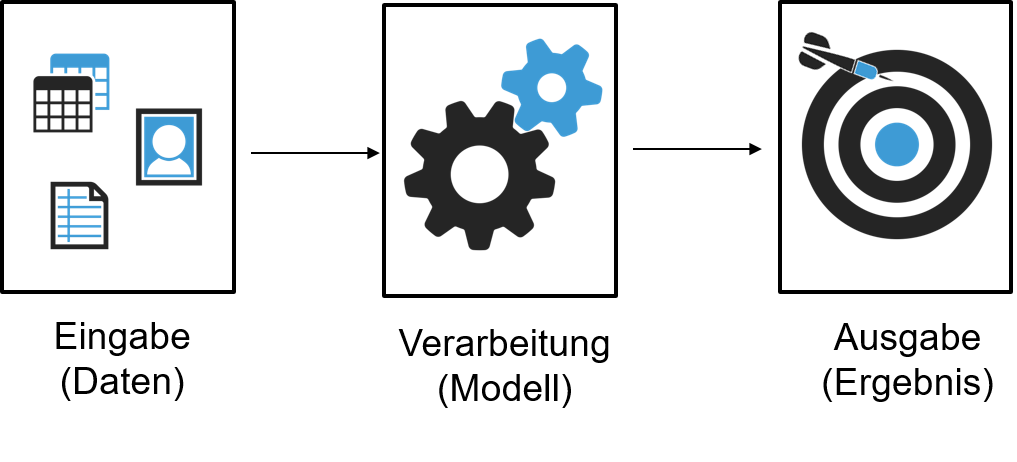
\includegraphics[width=12cm]{Bilder/data_bias.png}
		\caption{Machine Learning Pipeline: Eingabe, Verarbeitung, Ausgabe}
		\label{fig:dataBias}
	\end{center}
\end{figure}

\section{Daten}
\label{section:data}
\subsection{Unvollständigkeit der Daten}
\label{section:uncompleteData}
Unvollständige Daten sind Trainingsdatensätze, die z.B. nur einen Teil der Bevölkerung umfasst, während ein anderer Teil unterrepräsentiert ist. Dies nennt man Stichproben-Voreingenommenheit.
\\\\
Ein Beispiel dafür lieferte Apple 2017 mit der damals neuen FaceID des IPhone X.
Diese konnte zu Beginn durch Zwillinge, 3D Masken oder auch eng verwandte Personen ausgetrickst werden. Das größte Problem hierbei war allerdings, dass die Software mit Trainingsdaten trainiert wurde, bei der eine komplette ethische Gruppe unterrepräsentiert war. So konnten nicht miteinander verwandte Chinesen das selbe Handy entsperren und machten somit die Nutzung der FaceID unsicher\cite{iphone}.
%%% Übergang optional :)

\subsection{Garbage in - Garbage out}
\label{section:DataGarbage}
Eine Maschine kennt grundsätzlich keinen Unterschied zwischen Schwarz und Weiß, Mann und Frau oder Jung und Alt. Erst durch das Trainieren einer KI lernt eine Maschine Verhalten und Muster zu differenzieren. Hierfür werden qualitativ hochwertige Daten (siehe \ref{section:DataQuality}) benötigt, um das Netz richtig einzustellen.
\\\\
Bleiben fehlerhafte Daten unentdeckt, wird ein System falsche trainiert. In Testreihen für autonomes Fahren in der Autoindustrie kennzeichneten Probanden auf Grund von Unachtsamkeit, Menschen am Straßenrand als Tonnen ab. Das System wurde mit solcher Fehlkennzeichnungen trainiert und wertete in einer kritischen Verkehrssituation das Überfahren einer vermeintlichen Tonne als verhältnismäßigen Alternative ein, die möglichst wenig Schaden anrichtet \cite{trainingsDataKI}.
\\\\
Bei der traditionellen Datenanalyse können solche schlechte Daten nachträglich entfernt werden. Hat allerdings eine Maschine durch maschinelles Lernen etwas gelernt, wird es schwer dies wieder zu verlernen. Denn ähnlich wie beim menschlichen Gehirn, wird es ab einem Gewissen Grad nahezu unmöglich, herauszufinden, auf welche Datenelemente die Vorhersagen basieren.\\
Baut unser erlerntes Wissen in Teilen auf falsche Informationsbausteinen auf, verliert der ganze Komplex seinen Wert und man muss alles von vorne beginnen.
\\\\
Dieses Problem wird in der KI als "Garbage in - Garbage out" (Müll rein, Müll raus) bezeichnet.

\subsection{Historische Verzerrung}
\label{section:biasInTest}
Eine historische Verzerrung liegt vor, wenn ein Algorithmus anhand eines alten Datensatzes trainiert wird, der vergangene Werte und Moralvorstellungen etwa die Rolle der Frau in der Vergangenheit aufgreift\cite{kipedia}.
\\\\
Ein Beispiel liefert Amazons Algorithmus aus dem Jahr 2014, der unter mehreren Bewerbungstexten automatisch die besten Bewerber herausfiltern sollte. Dabei bezog die Software sich auf voran gegangene Bewerbungen, lernte daraus, welche Eigenschaften Amazon bevorzugte. Weil das Unternehmen aber Teil einer von Männern dominierten Industrie ist, sind in den zugrunde gelegten vergangenen zehn Jahren vor allem Männer eingestellt worden. Daraus resultierte, dass Frauen grundsätzlich schlechter bewertet wurden. Selbst ohne Angabe eines Geschlechtes wurden Frauen durch Frauenvereine identifiziert und kategorisch ausgeschlossen. Dies veranschaulicht das Problem der historischen Verzerrung, welches beim maschinellen Lernen in den Daten auftreten kann\cite{amazon}.
\\\\
Die Hoffnung solcher Anwendungen liegt eigentlich darin, Vorurteile zu vermeiden und Prozesse fairer zu gestalten, da eine Maschine wie in \ref{section:DataGarbage} bereits genannt, grundsätzlich keine Unterschiede kennt.
\\\\
An diesem Beispiel wird allerdings deutlich, wie zentral die Daten für eine KI sind.
Meist ist es nicht möglich Daten zu finden, welche nicht bereits menschliche Bias beinhaltet. Solch verzerrte Trainingsdaten, werden unter Bezug auf ihre Zusammensetzung auch als WEIRD Samples (western, educated, industrialized, rich and democratic societies) bezeichnet\cite{BiasInKi}.

\subsection{Under-/ Overfitting}
\label{section:OverUnderfitting}

Ein komplexer Datensatz (siehe Absatz \ref{section:DataQuantity}) kann beim überwachten Lernen dazu führen nutzloses Wissen aufzubauen oder aus einem vorhandenem Trainingsdatensatz keine relevanten Lerninformationen gezogen wurden. %%% 'ziehen zu können' oder 'gezogen wurden' überprüfen
Dies passiert, wenn ein Netz zu gut oder zu schlecht trainiert wurde. Diese Phänomene werden als Overfitting (Überanpassung) und Underfitting(Unteranpassung) bezeichnet.

\begin{figure}[h]
	\begin{center}
		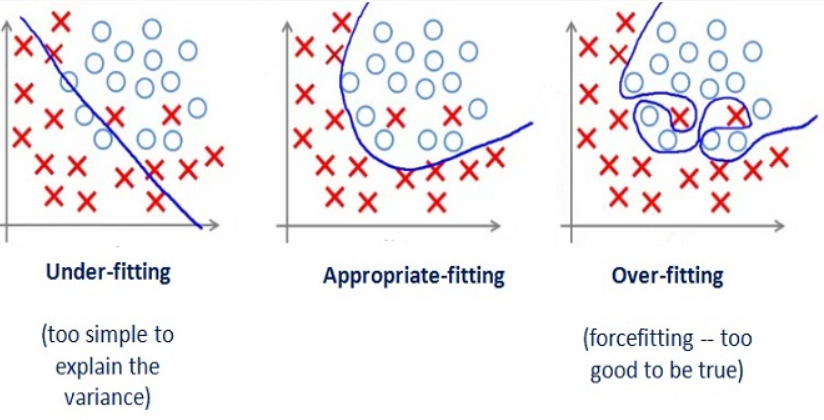
\includegraphics[width=12cm]{Bilder/overUnderfitting.png}
		\caption{Over- und Underfitting\cite{overUnderfitting}}
		\label{fig:overUnderFitting}
	\end{center}
\end{figure}

Die Abbildung \ref{fig:overUnderFitting} zeigt drei Graphen, die das Problem erläutern. Jeder Graph visualisiert abstrakt, wie unterschiedlich das KI-System anhand der Trainingsdaten, die einzelnen Punkte in zwei Cluster unterteilt. Die ''x'' und ''o'' stellen die zugewiesenen Kategorien durch den Menschen dar.
\\\\
Die KI im linken Graphen ist unter angepasst, da das Modell mit den Trainingsdaten zu schlecht abgestimmt wurde. Hier wurden zu wenig Punkte richtig abgedeckt, da die Funktion zu schwach ist um eine Generalisierung zu erreichen. Solche KI-Modelle neigen zu hohen Verzerrungen der Ergebnisse und teilt die einzelnen Trainingsdaten nur oberflächlich ein.
% Hier wurden zu wenig Punkte richtig abgedeckt, da zu wenige Muster zwischen den Eigenschaften und dem Label erkannt wurden. Solche KI-Modelle neigen zu hohen Verzerrungen der Ergebnisse und teilt die einzelnen Trainingsdaten nur oberflächlich ein.
\\\\
Der rechte Graph hingegen kategorisiert alle Punkte richtig ein. Unter dieser Annahme könnte man denken, es wäre der beste Graph. Hier spricht man allerdings von einer Überanpassung, da die Trainingsdaten zu stark auswendig gelernt und zu wenig generalisiert wurden. Verantwortlich dafür ist die Integration der Outliner(Ausreißer), die starke Abweichungen der eigenen Kategorie beinhalten. Solche Modelle besitzen eine hohe Varianz der Vorhersagen\cite{overUnderfitting}.
%da das Modell zu gut auf die Trainings- und Testdaten abgestimmt wurde. In der Praxis liefert dieses Model schlechte Ergebnisse. Verantwortlich dafür ist die Integration der Outliner, die starke Abweichungen der eigenen Kategorie beinhalten. Solche Modelle besitzen eine hohe Varianz der Vorhersagen\cite{overUnderfitting}.
\\\\
Beispielsweise wird eine KI mit Deep Learning darauf trainiert, einen Schrank auf einem Bild zu erkennen. Ist das KI-System über angepasst, beinhaltet es zu viele Eigenschaften der Ausreißer beispielsweise Sessel ähnliche Schränke. Das KI-Programm erkennt alle Trainings- und Testdaten perfekt, sobald man jedoch anfängt mit realen Daten zu testen, ist das Programm bei überschneidenden Eingaben sehr fehleranfällig. Outliner ähnliche Daten, wie in diesem Beispiel ein normaler Sessel, werden vom Programm als Schränke fehlinterpretiert, da das Modell zuvor über angepasst wurde. \\
\\\\
Am besten ist somit der mittlere Graph, welcher Outliner ignoriert und eine gute Balance zwischen Verzerrung und Abweichungen besitzt. 
\subsection{Aufteilung der Daten}
\label{section:AufteilungDerDaten}
Bei der Aufteilung von Trainings- und Testdaten können explizite Fälle nur in den Trainingsdaten auftreten. Zwar werden diese Fälle antrainiert, dadurch dass sie in den Testdaten fehlen nicht validiert. Das Netz liefert sehr gute Testergebnisse, jedoch nur da diese speziellen Fälle nicht getestet wurden. Diese fallen meist erst in der Praxis auf.
\subsection{Ähnlichkeit der Daten}
\label{section:similarData}
\begin{figure}[h]
	\begin{center}
		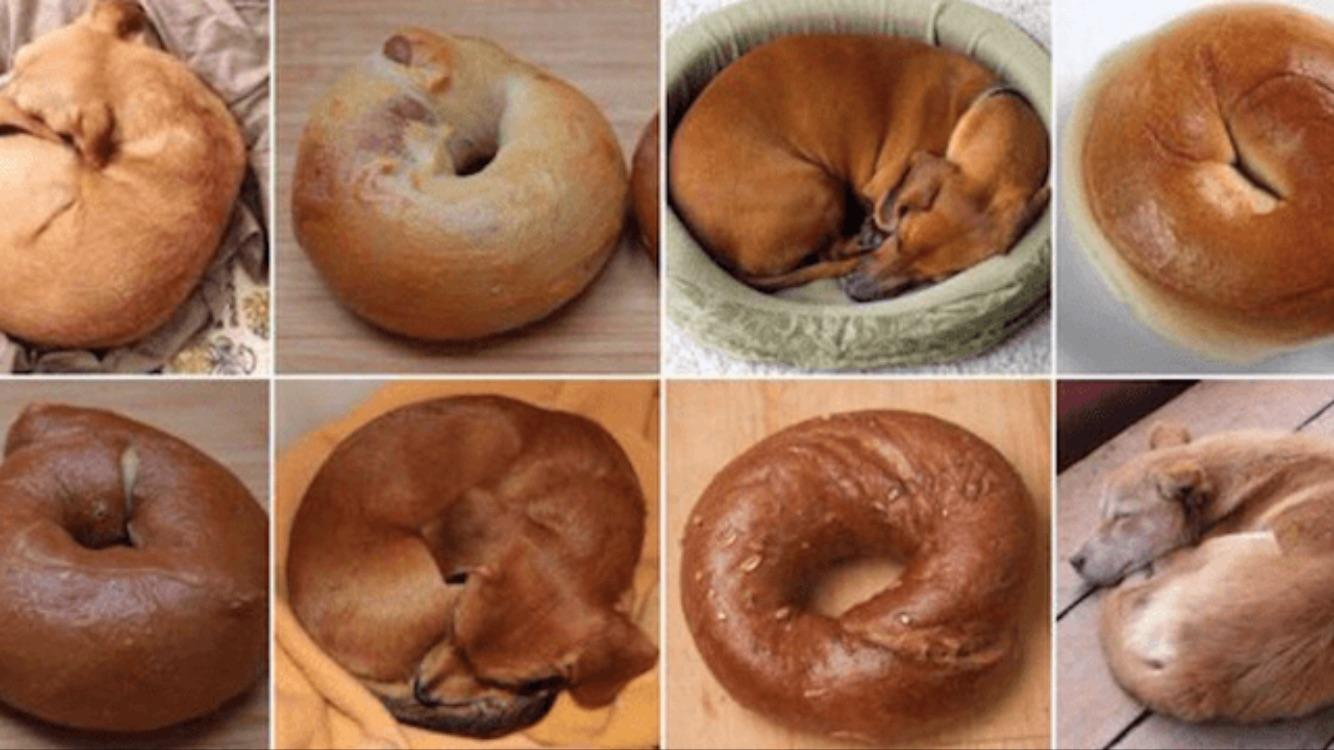
\includegraphics[width=15cm]{Bilder/dog_or_bagel.jpg}
		\caption{Hund oder Bagel?}
		\label{fig:dogBagel}
	\end{center}
\end{figure}

Optische Täuschungen sind Bilder, die Menschen in die Irre führen können. 
Anhand des Beispiels aus der Abbildung \ref{fig:dogBagel} wird deutlich,
dass wenn die Farbe, Struktur und die Form identisch sind,
die Wahrnehmung trüben kann. Ein Bagel wird auf den ersten Blick zum Hund oder andersrum. 
Das gilt auch für eine KI, denn das Programm lernt anhand Muster, Strukturen und sonstige besondere Eigenschaften zu kategorisieren. Hier kann es auch ohne falsche Eingaben zu einer Verzerrung der Ergebnisse führen.

\section{Menschliche Fehler}
\label{section:humanFehler}
Den Faktor Mensch darf man bei der Bias Entstehung nicht vergessen. Konzeptionelle Fehler, mangels an Wissen oder einem Missgeschick heraus, fördern Fehlverhalten. Markante Defizite können eine funktionale KI Entstehung komplett verhindern, sind jedoch in der Regel noch die besseren Missstände. Denn kleinere Mängel, die nicht sofort auffallen, können in Produktion fatale Folgen haben. %%% Nochmal drüberlesen, ob verständlich
\subsection{Falsche Zielsetzung}
Die Zielsetzung eines KNNs ist ein nicht zu unterschätzender Teil bei der KI Entwicklung. Setzt man hier den falschen Grundstein, können sich vermeidbare Fehlverhalten einer KI entwickelt.
\subsubsection{Subjektive Ziel Definition}
Eine Zielvariable spiegelt eine Antwort einer Frage wieder, die eine KI lösen soll. Wenn die Aufgabe lautet, findet den besten Mitarbeiter, muss die Zielsetzung in messbare Werte übersetzt werden. Bei dieser Definition kann bewusst oder unbewusst Bias eingepflegt werden. Anhand welcher Werte der 'Beste' Mitarbeiter erkannt wird, liegt allein an der subjektiven Meinung des Entwicklers. Ist die Meinung 'männlich, jung, intelligent' würde die KI Frauen diskriminieren \cite{KIPediaBias}.
% https://www.lernen-wie-maschinen.ai/ki-pedia/was-ist-algorithmische-voreingenommenheit-algorithmic-bias/
\subsubsection{Zu viele Ziele}
Viele Köche verderben den Brei. Diese Weisheit kann auch auf die Ziele von KNNs umgemünzt werden. Denn je mehr Ziele ein KNN hat, desto größer und komplexer muss ein künstliche neuronales Netz sein, um alle Fälle abdecken zu können. Je komplexer ein KNN ist, desto größer ist die Wahrscheinlichkeit, dass Fehler passieren. Auch ist sich das Netz deutlich unsicherer bei seinen Entscheidungen.
\\\\ % Ohne Quelle :(
Wenn man eine nahezu perfekte KI mit einer Aufgabe erweitern möchte, hat das meist zu Folge, dass die KI nach der Erweiterung zwar mehr kann, jedoch seine ehemalige Hauptaufgabe nicht mehr so gut meistert wie zuvor.
% Beispiel: Baidu Gesichtserkennung (erkennt nur Asiaten)
%%% Maybe ref Overfitting 
% \subsection{Falsches Lernen}
%%% Bescheibung nur bei Zeichennot
% Panzer Beispiel von oben, fällt in die Kategorie 'Falsches Lernen' mit ein
% Unvollständigkeit lieber mit dem Beispiel von Gesichtserkennung iPhone nehmen
% KI lernt oft einfachste Unterschiede
% \\i.	Nicht Unterschied zwischen Auto und Boot sondern Untergrund(Wasser/Land)
% \\ii.	Sehr Fehleranfällig z.B. Auto fährt durch flaches Wasser (KI -> Boot)
% \\iii. 	Mensch soll Lernprozess kontrollieren, ob KI auf dem richtigen Weg befindet
\subsection{Bewusste Manipulation der Trainingsdaten}
\label{section:manipulationInData}
Vorsätzliches Manipulieren von Trainingsdaten provoziert bewusst Fehlverhalten. Bei geschickter Manipulation ist der Betrug in den Datensätzen nicht erkennbar. Auch die KI funktioniert erwartungsgemäß. Nur bei bestimmten Eingaben tritt ein unerwünschtes Verhalten auf \cite{KIPediaBias}. \\\\
Vor allem bei öffentlichen Datensätzen kann man nicht hundertprozentig sicherstellen, dass keine Manipulation an den Daten vorgenommen wurden .
%%% Chat-Bot Tay bei Zeichennot
\chapter{Sicherheitsprobleme durch BIAS}
\section{Gefahren für Maschinen}
Computer, die von Computern gesteuert werden, sind heutzutage keine Science Fiction mehr. In der Industrie 4.0 nimmt KI eine immer größere Rolle ein. Somit können Fehlverhalten nicht nur Menschen sondern auch Maschinen schaden.
\subsubsection{Kühlung von Rechenzentren}
Seit 2016 setzt Google eine KI zur Optimierung des Kühlungsprozesses ein. Anfangs lieferte die KI nur Konzepte zur Kühlungsoptimierung, welche Mitarbeiter auswerten und einsetzt konnten. Heutzutage nimmt die KI Änderungen autonom an der Kühlung vor. Bis zu 40 Prozent an Energie konnte somit eingespart werden, was sich einerseits aus ökonomischer und als auch auf finanzieller Sicht lohnt \cite{GoogleKI}.\\ 
% Der Teil ist rein spekulativ und nicht belegbar
Unterläuft der KI hier ein Fehler, hat dies direkte Folgen auf die Langlebigkeit der Computerelemente des Rechenzentrums und kann sogar zu Brandherden in Gebäuden führen.
\section{Gefahren für Menschen}
In Zukunft werden KIs immer mehr zu unseren Alltag gehören und greifen immer stärker in unseren Leben ein. Dies hat viele Vorteile, jedoch ebenso Nachteile insbesondere für ärmere Teile der Bevölkerung sowie Minderheiten.
%%% Übereinleitung kann auch gestrichen werden
\subsection{Diskriminierung von bestimmten Personengruppen oder Minderheiten}
Einleitungsvariante 1 \\
Alltagsrassismus ist ein Denkschemata größerer sozialen Gruppen, die ein 'Wir' konstruieren und andere insbesondere Minderheiten kategorisch ausschließen oder andersartig benachteiligen.\\
Dieses Kategorisieren ist einer der Hauptfunktion der KI. Dadurch werden schnell bewusst oder unbewusst Diskriminierungen eingepflegt. Was das für Auswirkungen heute schon hat, zeigen folgende Beispiele.
\\\\ Einleitungsvariante 2\\
Durch die \#BlackLivesMatters Bewegung 2020 ist die Forderung nach Gleichberechtigung aktuell wieder omnipräsent. KI könnte hier abhelfen. Denn KIs sind Programme und können somit keine Vorurteile besitzen. Leider ist die Theorie nur eine Halbwahrheit. Natürlich sind Algorithmen von sich aus nicht rassistisch Motiviert, jedoch spiegeln sie diskriminiertes Verhalten aus Daten oder sonstigen Fehlern heraus wider.
\subsubsection{Alltagsrassismus}
Amazon entwickelte 2014 ein Bewerbungsauswahlsystem, wie bereits in \ref{section:biasInTest} beschrieben. Dort hat die KI empfohlen nur Männer einzustellen. \\\\
In Finnland wurde Svea Ekonomi ein Onlinekreditvergabe Unternehmen auf 100.000 Euro Strafe verurteilt, aufgrund eines Falles von direkter Mehrfachdiskriminierung. Der Antragssteller wurde ein Verlängerung des Kredits verweigerten ohne Berücksichtigung des Kreditverhaltens und Kreditwürdigkeit. \\Allein basierend auf statistische Zusammenhänge von Faktoren wie Geschlecht, Muttersprache, Alter und Wohnort wurde ein Score berechnet, auf dem die Kreditwürdigkeit beruht. \\Männer wurden schlechter bewertet als Frauen, auch wurden schwedische Muttersprachler besser bewertet als finnische. Da der finnisch sprechende Antragssteller aus einem für das System unbekannten Gebiet kam, welches ebenso eine Benachteiligung darstellt, wurde der Kredit verweigert. Statistisch gesehen, ist es korrekt, dass junge finnische Männer, die aus einer schlechteren Gegend kommen, häufiger Rückzahlungsprobleme haben. Jedoch diese Daten zu verallgemeinern und ohne auf individuelle Berücksichtigung des Kreditverhaltens und Kreditwürdigkeit einzugehen, ist schlicht weg diskriminierend. 
Wäre nur ein Faktor, arithmetisch gesehen, günstiger für den männlichen Antragssteller gelegen, hätte er den Kredit bekommen \cite{DiskriminierungKredit}.

\subsubsection{Risikobeurteilung}
In Amerika wird eine KI namens COMPAS eingesetzt, um Risikobeurteilung von Angeklagten und Häftlingen zu erstellen. Benachteiligt werden eindeutig Minderheiten. Nachweislich lag die Software doppelt so oft mit den Prognosen zukünftiger Verbrechen von Afroamerikanern falsch im Vergleich zu weißen Angeklagten. %%% Passt der Satz so?
Durch schlechte Sozialprognosen haben afroamerikanische Angeklagte eine geringe Chance auf frühzeitige Entlassung oder auf Bewährung. Bedeutet, afroamerikanische Straftäter müssen durchschnittlich länger Inhaftieren als Weiße, dank KIs.
%%% evtl. ref auf Historische Verzerrung 
\subsection{Lebensgefahr}
Tesla und Volvo prognostizierten 2015, dass 2017 vollständig autonome Fahrzeuge marktreif wären. Das Fraunhofer-Institut prophezeit 2025 als frühesten Zeitpunkt, während die Deutsche Akademie der Technikwissenschaften 2030 nennt \cite{AutonomAuto}.
\\Trotzdem schickt Tesla seine Kunden mit einer unausgereiften KI autonom auf die Straßen. Allein mit dem Zweck Daten zu sammeln. Dass in Verbindung mit autonomen Fahren immer wieder Unfälle bis hin zu Todesfällen gemeldet werden, zeigt, dass künstliche Intelligenz unmittelbare Konsequenzen für den Mensch mit sich bringt. \\\\
Ein Beispiel für die Unausgereiftheit ist dieses Verkehrsschild. %%% Unausgereiftheit?
\begin{figure}[h]
	\begin{center}
		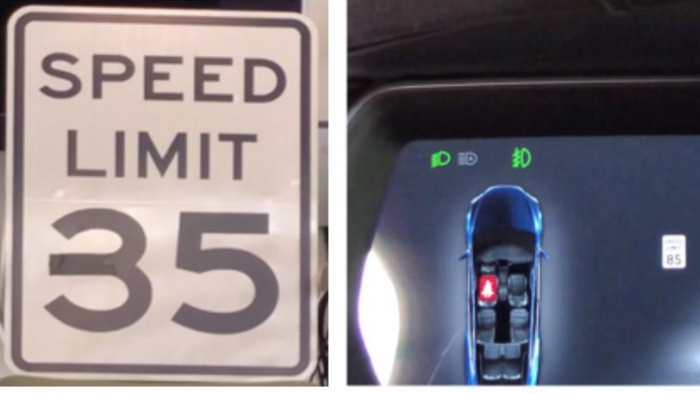
\includegraphics[width=15cm]{Bilder/Tesla_Adversarial_Attack.png}
		\caption{35 oder 85 mph?}
		\label{fig:Verkehrsschild}
	\end{center}
\end{figure}
Die Geschwindigkeitsbegrenzung wurde bewusst manipuliert und indem das mittele Teil der Drei verlängert wurde. Teslas KI erkannte die Drei als Acht und beschleunigte automatisch um mehr als 80 km/h. Diese bewusste Manipulation nennt man Adversarial Attacks \cite{TeslaHack}.
\section{Angriff auf KI}
Ist eine Künstliche Intelligenz sehr gut trainiert, erzielt sie in ihrem Aufgabebereich überragende Ergebnisse. Selbst nahezu perfekte KIs sind nicht unfehlbar. Durch methodisch gestaltete Störungen der Eingeben kann eine KI bewusst getäuscht werden und damit die Computer-Wahrnehmung in die Irre führen. Diese Art der Ausnutzung von KI Schwächen nennt man Adversarial Attacks, zu deutsch gegensätzlicher Angriff.
\subsubsection{Adversarial Attacks}
Bildererkennungssoftware ist besonders anfällig für dieser Art von Angriff. 
%%% ref auf fig:Verkehrsschild
Hierbei legt man über das Bild bestimmte Pixelmuster, die für das menschliche Auge in der Regel im Gesamtbild untergehen. KIs hingegen registrieren jegliches Muster und nehmen sie in ihre Berechnungen mit auf. Als Ergebnis werden Bilder zum Teil massiv fehlinterpretiert.
Im folgenden Angriff wird mit einer Brille und dessen speziellen Muster, eine KI überlistet.
\label{section:BrilleAttack}
\begin{figure}[h]
	\begin{center}
		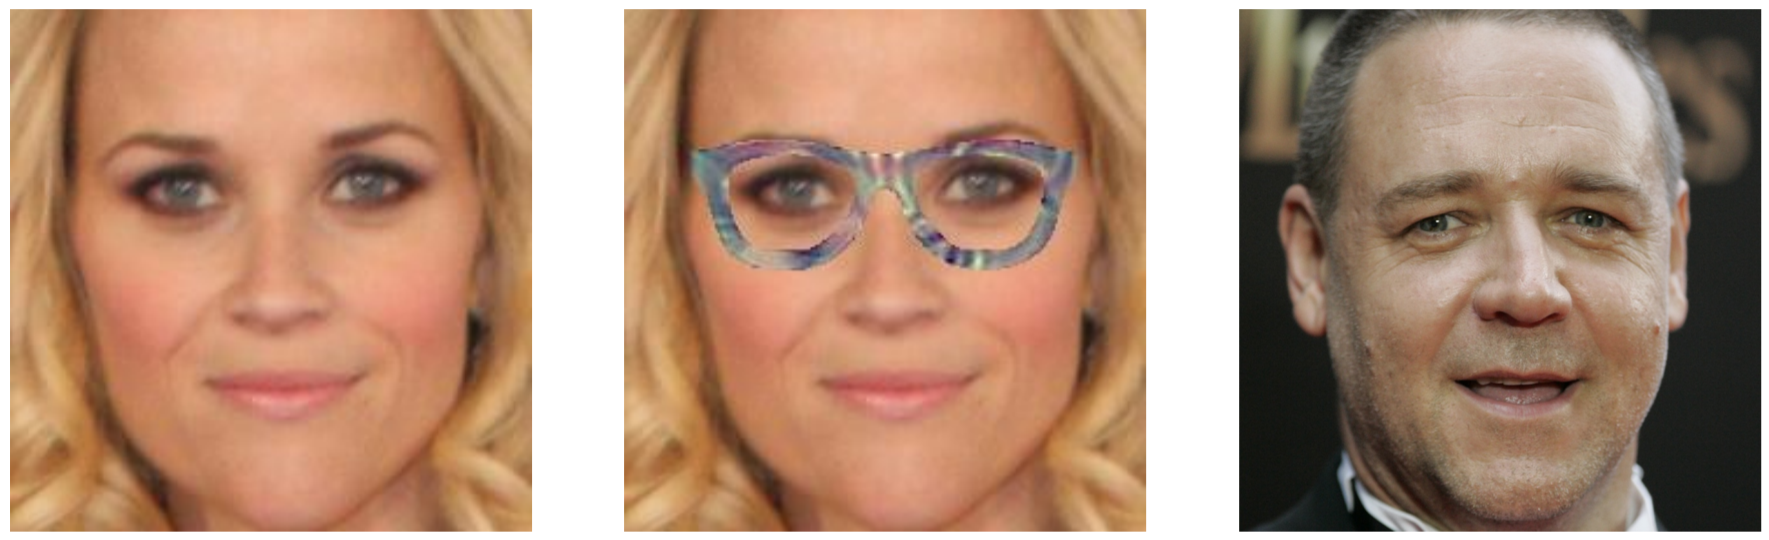
\includegraphics[width=15cm]{Bilder/Brille_Adversarial_Attack.png}
		\caption{Reese Witherspoon wird mit Adversarial Attack Brille zu Russel Crowe}
		\label{fig:BrilleAttack}
	\end{center}
\end{figure}
% Paper https://www.cs.cmu.edu/~sbhagava/papers/face-rec-ccs16.pdf
\\Im linken Bild sieht man die amerikanische Schauspielerin Reese Witherspoon. Dieses Bild wird auch korrekt als sie selbst von der KI erkannt. Setzt man ihr eine spezielle Brille auf, beginnt das neuronale Netz Fehler zu begehen. Plötzlich erkennt die KI Reese Witherspoon mit der Brille als Russel Crowe (Bild rechts) \cite{Attack}.

\chapter{Prävention}
\label{chapter:main}
\section{Passender Algorithmus zu Daten}

Ab einem gewissen Grad ist es schwer ein bestehendes Modell, dass mit fehlerhaften Daten trainiert wurde, das Fehlverhalten zu verstehen und zu entfernen, siehe Abschnitt \ref{section:DataGarbage}.
\\\\
In der Annahme, ein KI-System wurde richtig trainiert, aber die zeitliche Komponente nicht beachtet, kann es zu einer historischen Verzerrung \ref{section:biasInTest} kommen.
Wie Stöcker 2019 \cite{stoecker} bereits erwähnte, benötigt eine sich ändernde Gesellschaft auch kontinuierliche weiterlernende Algorithmen. Solch ein Lernprozess wird auch als \textit{adaptive learning} bezeichnet, womit dem Effekt sich ändernder Datenumgebungen(concept drift) Rechnung getragen wird \cite{gama}.%%% Vll nochmal ansprechen
\\\\
Auch bei einem für Diskriminierung anfälligen Umfeld muss besondere Sorgfalt bei der Wahl des passenden Algorithmus bedacht werden. In der Regel reicht es einzelne Attribute aus den Eingangsdaten auszuschließen, um eine algorithmische Diskriminierung bestimmter Personengruppen zu verhindern. Dies genügt jedoch oftmals nicht, denn wie das Beispiel von Amazon aus \ref{section:biasInTest} zeigt, kann der Algorithmus Rückschlüsse anhand anderer Attribute ziehen(z.B. durch Frauenvereine).
\\\\
In diesem Kontext sollten KI-System bevorzugt werden, welche in der Entwicklung zusätzliche Einschränkungen einführen, um eine Diskriminierung aufgrund bestimmten Attributen zu verhindern \cite{kamiran}.

\section{Nur ein Ziel}
\label{section:oneGoal}

Generell ist es zu empfehlen mehrere spezialisierte KIs für einzelne Aufgaben zu verwenden, anstatt einer KI immer mehr Aufgaben aufzulasten. Je konkreter und einfacher die Aufgabe und dessen Zielsetzung gehalten wird, desto fehlerfreier kann eine KI die Aufgabe lösen.\\\\
Setzt man sich zu hohe Ziele, kann das komplexe System leicht unter trainiert oder übertrainiert werden, siehe Abschnitt \ref{section:OverUnderfitting}. Man braucht dementsprechend exorbitant mehr Datensätze zum Trainieren des Netzes und bei denen man auch leicht historische Verzerrungen \ref{section:biasInTest} oder Manipulationen \ref{section:manipulationInData} übersehen kann.
\section{Verfahren zum Validieren}
\label{section:validate}

Damit menschliche Fehler (Abschnitt \ref{section:humanFehler}) oder fehlerhafte Daten (Abschnitt \ref{section:Data}) frühzeitig erkannt werden und nicht zu Fehlern führen, sollten diese zuvor validiert werden. Folgende Verfahren wirken menschliche Fehler entgegen:
\begin{enumerate}
	\item Lektorat oder Peer-Review
	\item Das Vier-Augen-Prinzip
	\item Mehrheitsentscheide bei unterschiedlichen Ergebnissen
\end{enumerate}
Die oben genannten Verfahren bekämpfen Flüchtigkeitsfehler und bewusste Manipulation. Beim Peer-Review kontrollieren nachträglich Experten das KI-System auf dessen Korrektheit. Beim Vier-Augen-Prinzip und bei Mehrheitsentscheide passiert dies während des Arbeitsprozesses. 
\\\\
Zudem sollte das KI-System ausreichend auf Fehleranfälligkeit geprüft werden. Vor allem im kritischen Bereichen, wie in der Medizindiagnostik, sollten die Fehleranfälligkeit gegen null gehen. Anhand des Problem aus Abschnitt \ref{section:AufteilungDerDaten}, können ungeprüfte Fälle fehlerhaft sein.
\\\\
Eine Möglichkeit um das zu verhindern, bietet die Kreuzvalidierung. 
\begin{figure}[h]
	\begin{center}
		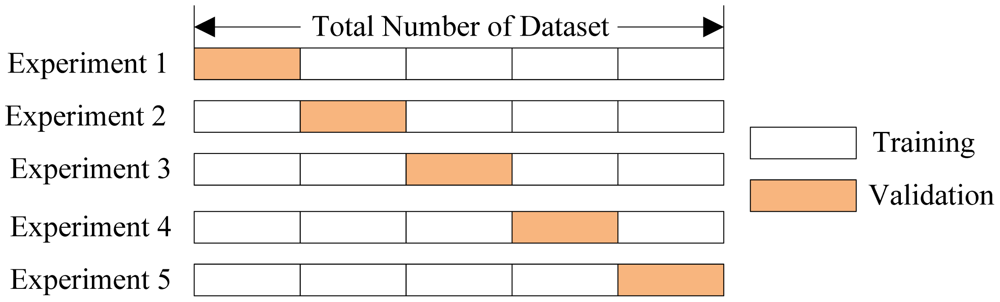
\includegraphics[width=15cm]{Bilder/crossValidierung.png}
		\caption{fünf fache Kreuzvalidierung}
		\label{fig:crossValidierung}
	\end{center}
\end{figure}
\\Anstelle eines fixen Testdatensatzes wird der komplette Datensatz in viele kleine Blöcke unterteilt, in der Abbildung \ref{fig:crossValidierung} Fünf. In diesem Beispiel werden fünf Durchläufe ausgeführt, in denen jeweils abwechselnd mit vier unterschiedlichen Datensätzen trainiert und mit einem validiert wird. Bei jedem Durchlauf entsteht ein Score über die Fehleranfälligkeit. Am Ende wird ein durchschnittlicher Score über diese fünf Durchläufe gebildet, welcher die gesamt Fehleranfälligkeit für alle Datensätze wider gibt.
\\\\
Mit Hilfe der Kreuzvalidierung lässt sich eine Aussage treffen, wie gut das Modell mit unbekannten Daten trainiert. Dieses Prinzip nennt man die Generalisierung.

\section{Over- und Underfitting}
\label{section:preventData}
Die Kunst der Modellierung besteht darin, ein optimales Modell(siehe mittleren Graphen \ref{fig:overUnderFitting}) zu finden, dass eine perfekte Balance zwischen Verzerrung und Abweichung der Daten besitzt. Dieses Modell sollte eine so gering wie mögliche Komplexität und gut beschriebene und generalisierte Daten haben. Da das nicht immer einfach zu erreichen ist, treten Underfitting und Overfitting auf, siehe Abschnitt \ref{section:OverUnderfitting}.

\subsection{Underfitting}
Underfitting ist die Folge eines zu einfachen Modells und liefert somit schlechte Vorhersagen. Eine Möglichkeit um dies zu verhindern ist das Erhöhen der Flexibilität. Dass heißt die Anzahl an Merkmalen die einen Datensatz auszeichnen und die Menge der Trainingsdaten müssen erhöht werden. Eine weitere Möglichkeit bietet das Erhöhen der Durchläufen beim Trainieren der Trainingsdaten.

\subsection{Overfitting}
Overfitting stellt in der KI eine große Herausforderung dar und ist die Folge aus einem zu komplexen Modell. Eine Möglichkeit um eine Überanpassung zu vermeiden, bietet eine Resampling Methode, wie z.B. die Kreuzvalidierung, siehe Abschnitt \ref{section:validate}. 
Eine andere Methode ist die Vereinfachung des Ki-Systems. So kann mit Hilfe von Pruning die Größe eines Bäumen reguliert werden\cite{overUnderfittingNovu}. Bei Regressionsmodellen hingegen können Regulierungstechniken angewandt werden.
\\\\
Bei der Regulierung wird ein Strafterm eingeführt, der die Anzahl an Variablen und deren Wechselwirkungen berücksichtigt(siehe Abbildung \ref{fig:regFunc}).

\begin{figure}[h]
	\begin{center}
		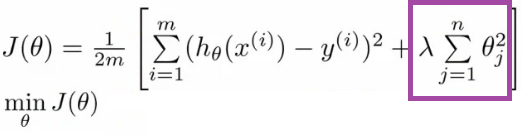
\includegraphics[width=10cm]{Bilder/regFunc.png}
		\caption{Regularisierung in Loss Funktion}
		\label{fig:regFunc}
	\end{center}
\end{figure}
Wenn in der Abbildung \ref{fig:regFunc} die Komplexität steigt, wird eine Strafe hinzugefügt. Das hat zur Folge, dass die Wichtigkeit solcher langen Terme sinkt und zugleich die Komplexität des Models weniger wird.
\\\\
Beispiele für solche Techniken sind folgende:
\begin{enumerate}
	\item L1 Regulierung (Lasso Regulierung)
	\item L2 Regulierung (Ridge Regulierung)
	\item Elastic net
\end{enumerate}

\chapter{Fazit}
Die künstliche Intelligenz ist weiterhin auf den Vormarsch. So wundert es nicht, dass sich immer mehr Unternehmen mit dieser Technologie beschäftigen. Die Nutzung birgt jedoch das Risiko, KI Bias zu erzeugen, welche im schlechtesten Fall zu hohen Kosten führen können. Diese Arbeit beschäftigte sich daher mit der Entstehung solcher Bias und wie diese verhindert werden können.
\\\\
Die Datenaufbereitung ist ein zentrale Grund für den Erfolg einer KI. Ohne diese können zahlreiche Bias entstehen. Die Folgen dieser Verzerrungen sind Sicherheitsrisiken für einzelne Gruppen oder Geschlechter. Die Kosten solcher Fehlimplementierungen können sehr hoch, aber mit z.B. guter Datenqualität vermeidbar sein.
\\\\
Es gibt viele Forscher, die sich mit solchen Themen beschäftigen und gezielter auf einzelne Bias eingehen. In dieser Arbeit war der Hauptaugenmerk allerdings auf die allgemeine Entstehung solcher Bias und welche Sicherheitsprobleme dadurch auftreten können.
\\\\
Noch mehr gefährliche Auswirkungen auf Gesellschaft und Demokratie beschreibt Norbert Lossau in seiner Analyse über Deep Fake\cite{deepFake}. DeepFakes sind manipulierte Videos, in denen Personen erfundene Aussagen in den Mund geschoben werden oder in denen sie scheinbar Handlungen begehen, die in Wirklichkeit nie stattgefunden haben. Diese Fakes werden immer besser, so dass diese kaum noch zu erkennen sind. Die Sicherheitsrisiken für die Menschen sind somit durchaus größer als hier beschrieben. Daher ist es sinnvoll Untersuchungen auf solche Thematiken auszuweiten.
\\\\
Diese Arbeit hat sich
Thema ist größer als hier beschreibbar
\\Evtl. Deep Fake
http://iphome.hhi.de/samek/pdf/LapNCOMM19.pdf
https://ujjwalkarn.me/2016/08/11/intuitive-explanation-convnets/


\backmatter
%%%%%%%%%%%%%%%%%%%
%% create tables list
%%%%%%%%%%%%%%%%%%%
%\listoftables

%%%%%%%%%%%%%%%%%%%
%% create listings list
%%%%%%%%%%%%%%%%%%%
%\lstlistoflistings
%\addcontentsline{toc}{chapter}{Listings}

\cleardoublepage
\phantomsection
\addcontentsline{toc}{chapter}{Literatur}
\printbibliography

\end{document}
